
% \usepackage{geometry}
\usepackage[dvipdfmx]{graphicx}
\usepackage{ascmac}
\usepackage{amsmath}
\usepackage{amssymb}
\usepackage{minted}
\usepackage{listings}
% \usepackage[utf8]{inputenc}
% \usepackage{listingsutf8}
\usepackage{newfloat} % newfloat パッケージを読み込む
\usepackage{caption}
\usepackage{float}
\usepackage{fix-cm}
\usepackage{svg}
\usepackage{enumitem}

\usepackage{hyperref}
% for hyperref
\usepackage{pxjahyper}
\hypersetup{
    dvipdfmx,
	colorlinks=false, % リンクに色をつけない設定
	bookmarks=true, % 以下ブックマークに関する設定
	bookmarksnumbered=true,
	pdfborder={0 0 0},
	bookmarkstype=toc
}

% \lstset{
%   basicstyle={\ttfamily},
%   identifierstyle={\small},
%   inputencoding=auto,
%   commentstyle={\small\sffamily},
%   keywordstyle={\small\bfseries},
%   ndkeywordstyle={\small},
%   stringstyle={\small\ttfamily},
%   frame={tb},
%   breaklines=true,
%   columns=[l]{fullflexible},
%   numbers=left,
%   % xrightmargin=0zw,
%   % xleftmargin=3zw,
%   numberstyle={\scriptsize},
%   firstnumber=auto,
%   stepnumber=1,
%   numbersep=5pt,
%   lineskip=1ex
% }

% 新しい浮動体「listing」を定義
\DeclareFloatingEnvironment[
    fileext=lol,       % List of Listings ファイルの拡張子 (List of Listings を作成する場合)
    name=Listing,      % キャプションの接頭辞 (例: "Listing 1")
    placement={!htbp}, % フロートの配置オプション (お好みで調整してください)
    within=section     % 番号付けをセクションごとにする場合 (例: Listing 1.1) (任意、不要なら削除)
]{program}

\setminted{
  mathescape,              % 数式モードへのエスケープを許可 (必要なら)
  % basicstyle やフォント関連
  fontsize=\small,         % 全体のフォントサイズ (listings の \small に合わせる試み)
                           % \ttfamily は minted のデフォルトに近いが、日本語対応の等幅フォントを
                           % LaTeX 側で \ normaalfont や \ttdefault に設定しておくのが理想
  % frame
  frame=lines,             % 上下に線を引く frame=tb に近いものとして lines (上下左右に線)
  framesep=2mm,            % 枠線とコードの間隔 (調整が必要)
  % breaklines
  breaklines=true,         % 自動折り返し
  % numbers
  linenos=true,            % 行番号を左に表示
  firstnumber=auto,        % 行番号を開始行に合わせる
  numbersep=5pt,           % 行番号とコードの間隔
  % stepnumber=1,          % linenos=true で通常1ステップ
  % highlight と Pygments スタイル
  % minted では Pygments のスタイルを使います。
  % style=friendly のようにスタイル名を指定できます。
  % デフォルトのスタイルでキーワードが太字になるか確認。
  % commentstyle や keywordstyle の LaTeX コマンド直接指定はできません。
  % Pygments のスタイルでこれらがどのように見えるか確認し、
  % 必要ならカスタムスタイルを作るか、別の既存スタイルを選びます。
}
% コピペフィニィッシュ
\title{C++入門}
\author{佐藤謙成}
\institute{KUT-PG}

\begin{document}
\begin{frame}
    \titlepage
\end{frame}

\begin{frame}{目次}
  \tableofcontents[sections={1-6}]
\end{frame}

\begin{frame}{目次(続き)}
    \tableofcontents[sections={7-12}]
\end{frame}

\begin{frame}{初めに}
    このC++入門では,プログラムの基本的な文法を学んでもらうことが目標である.既に習得済みの分野については飛ばしても問題はない.
    C++を完全に理解するためには参考書やyoutube等の活用をおすすめする.また,atcoder等のプログラム課題については積極的に取り組んでもらいたい.
\end{frame}

\begin{frame}{注意}
    このスライドはtexのbeamerというドキュメントクラスを用いています.
\end{frame}
\section{Hello Worldの出力}

\begin{frame}[fragile]{Hello world}
ここでは,プログラミング言語の最初の慣習としてHello worldの出力を行なっていく.
% \begin{minipage}{\linewidth}
    \lstinputlisting[caption=Hello.cpp, label=01]{code/hello.cpp}
% \end{minipage}
次のスライドからはこのソースコードの解説を行なっていく,
\end{frame}

\begin{frame}[fragile, allowframebreaks]{ソースコード\ref{01}の解説}
    \begin{block}{ヘッダーファイル}
        \lstinputlisting[basicstyle=\ttfamily\footnotesize]{./code/io.txt}
        このコードは,ヘッダーファイルと呼ばれる物である.
        このファイルを読み込むことにより,coutやcinを用いることができる.
    \end{block}
    \newpage
    \begin{block}{main関数}
        \lstinputlisting[basicstyle=\ttfamily\footnotesize]{./code/sorce.txt}
        各コードに必ず存在する特別な関数.
        プログラムはmain関数の最初から順に実行されていく.
        基本的には,main関数内に記述すれば良い.
        詳しくは\ref{main}ページで解説している.
    \end{block}
    \begin{block}{cout << "Hello World"}
        Hello Worldという文字列を出力している.
    
        詳しくは\ref{in_out}ページで解説している.
    \end{block}

    \begin{block}{プログラムの終了}
    \lstinputlisting[basicstyle=\ttfamily\footnotesize]{./code/return.txt}
    このコードを記述することでプログラムを終了することができる.
    (必要なくても実行が最後まで到達すればプログラムは終了する.)
\end{block}
\end{frame}


\section{変数}
\begin{frame}{変数とは}
    \begin{block}{変数}
        記憶域(メモリ)\footnote{そういうものがある程度の認識で大丈夫.}に名前をつけてさまざまな値を格納できるようにしたもの.
        変数は値を格納する箱という認識で大丈夫である.
    \end{block}
    \begin{table}[]
        \centering
        \begin{tabular}{|l|l|l|}
            \hline
            型       & キーワード  & サイズ\\
            \hline
            文字データ & char  & 1バイト\\
            符号付き整数 & int  & 4バイト\\
            浮動小数点 & float & 4バイト\\
            倍精度浮動小数点 & double & 8バイト\\
            値なし & void & \\
            \hline
        \end{tabular}
        \caption{基本のデータ型}
        \label{tab:my_label}
    \end{table}
\end{frame}

\begin{frame}{変数の宣言}
    変数をプログラム内で使用する際には変数の宣言というものが必要となる.
    \begin{block}{宣言方法}
        変数宣言の一般的な形式は次の通りである : \textbf{型 \mbox{ }変数名;}\footnote{int x, y, z; とまとめて宣言することもできる.}
        \mbox{}\\
        
        実際にコード内で書く例は次の通りである : \textbf{int counter\footnote{変数名は自身で設定することができるため,格納される値に沿った名前にすること.};}
    \end{block}
    \begin{alertblock}{}
        変数宣言は1つの文であるため,一番最後にセミコロン(;)が必要である.
        
        よく忘れるため注意すること.
    \end{alertblock}
        
    
\end{frame}
\begin{frame}{変数の種類}
    \begin{block}{グローバル変数}
    通常の関数やmain関数の外で宣言された変数.そのプログラム内のどの関数からも使うことができる.ただし,どこでどの手順で変数内の値が変更されたか不透明になりやすいため,基本的には使用を避けたい.
    \end{block}
    \begin{block}{ローカル変数}
        通常の関数やmain関数内で宣言された変数.宣言された関数内でのみ使用可能.変数内の値がどこでどの手順で変更されたか分かりやすい.
    \end{block}
\end{frame}
\begin{frame}{変数の代入}
    \begin{block}{代入方法}
        代入の一般的な形式は次のとおりである : 変数名 = 値;
        
        実際の例は次の通りである : count = 5;\footnote{int count = 5; のように変数の宣言と同時にすることができる.}
    \end{block}
\end{frame}
\section{入出力} 
\label{in_out}
\begin{frame}[fragile]{入出力}
    \begin{block}{入力}
        \lstinputlisting[basicstyle=\ttfamily\footnotesize]{./code/cin.txt}
    \end{block}
    \begin{block}{出力}
        \lstinputlisting[basicstyle=\ttfamily\footnotesize]{./code/cout.txt}
        \begin{itemize}
            \item endlで改行する.\footnote{"\textbackslash n"でも可能.}
            \item ""(ダブルクォーテーション)で囲んだ文字列はそのまま文字列のまま出力される.
        \end{itemize}
    \end{block}
\end{frame}

\section{プログラムの演算}
\begin{frame}{算術式の計算}
    \begin{table}[]
        \centering
        \begin{tabular}{|l|l|l|}
            \hline
            演算子 & 意味 & 優先順位\\
            \hline
            * & 乗算 & 4\\
            / & 除算(余りは切り捨て) & 4\\
            \% & 剰余 & 4\\
            + & 加算 & 5\\
            - & 減算 & 5\\
            \hline
        \end{tabular}
        \caption{算術演算子}
        \label{tab:my_label}
    \end{table}
    \begin{block}{}
        もし,加算・減算を先に求めたい場合は()を用いることで優先順位を上げることができる.
    \end{block}
\end{frame}

\begin{frame}{複合代入演算子}
    \begin{block}{}
        計算式の省略形.競プロではよく使用されるので覚えておきたい.
    \end{block}
    \begin{table}[]
        \centering
        \begin{tabular}{|l|l|}
            \hline
            複合代入演算子 & 代入演算子 \\
            \hline
            a += 1 & a = a + 1\\
            a -= 3 & a = a - 3\\
            a *= 5 & a = a * 5\\
            a /= 2 & a = a / 2\\
            a \%= 9 & a = a \% 9\\
            \hline
        \end{tabular}
        \caption{複合代入演算子}
        \label{tab:my_label}
    \end{table}
\end{frame}

\begin{frame}{インクリメント, デクリメント}
    \begin{block}{インクリメント}
        a++; または ++a;である.
        
        この二つは計算の優先順位が存在するため,式の途中で登場する場合は異なる結果となる.
    \end{block}
    \begin{block}{デクリメント}
        a--; または --a;である.
    \end{block}
    次のスライドで実際にどのように違うのか検証していきたい.
\end{frame}

\begin{frame}[fragile, allowframebreaks]{インクリメント,デクリメント}
    まずは,前置インクリメント\footnote{++aのこと.}のソースコードである.
    \begin{minipage}{\linewidth}
        \lstinputlisting[caption=Pre\_increment.cpp, basicstyle=\ttfamily\footnotesize]{./code/Pre_increment.cpp}
    \end{minipage}

    次は,後置インクリメント\footnote{a++のこと.}である.
    \begin{minipage}{\linewidth}
        \lstinputlisting[caption=Pos\_increment.cpp, basicstyle=\ttfamily\footnotesize]{./code/Pos_increment.cpp}
    \end{minipage}
\end{frame}

\begin{frame}{前置インクリメント, 後置インクリメント}
\begin{table}[]
    \centering
    \begin{tabular}{|l|l|}
    \hline
        演算子 & 説明\\
        \hline
       前置インクリメント  & 先に値をインクリメント(+1)した後に代入 \\
       後置インクリメント  & 先に代入した後に値をインクリメント(+1)\\
       \hline
    \end{tabular}
    \caption{前置,後置の違い}
    \label{tab:my_label}
\end{table}
    
\end{frame}

\begin{frame}{関係演算子}
この演算子は,数学等で頻繁に出るため,簡単に押さえておけばよい.
    \begin{table}[]
        \centering
        \begin{tabular}{|l|l|}
        \hline
        演算子 & 関係\\
        \hline
        > & より大きい\\
        >= & 以上\\
        < & より小さい\\
        <= & 以下\\
        == & 等しい\\
        != & 等しくない\\
        \hline
        \end{tabular}
        \caption{関係演算子}
        \label{tab:my_label}
    \end{table}
\end{frame}

\begin{frame}{論理演算子}
1年生の2Q(情報代数), 3Q(離散数学)で出てくるため押さえておきたい.
    \begin{table}[]
        \centering
        \begin{tabular}{|c|l|}
        \hline
        演算子 & 操作\\
        \hline
        \&\& & 論理積(かつ)\\
        || & 論理和(または)\\
        ! & 否定\\
        \hline
        \end{tabular}
        \caption{論理演算子}
        \label{tab:my_label}
    \end{table}
    \begin{table}[]
        \centering
        \begin{tabular}{|c|c|c|c|c|}
        \hline
        p & q & p \&\& q & p || q & !p\\
        \hline
        T & T & T & T & F\\
        T & F & F & T & F\\
        F & T & F & T & T\\
        F & F & F & F & T\\
        \hline
        \end{tabular}
        \caption{真理値表}
        \label{tab:my_label}
    \end{table}
\end{frame}

\section{条件分岐}
\begin{frame}[fragile]{条件分岐を用いたソースコード}
    ここに載せているソースコードは条件分岐を用いた実際のコードである.詳しい解説は次からのスライドで行う.
    \begin{minipage}{\linewidth}
        \lstinputlisting[caption=if.cpp, basicstyle=\ttfamily\footnotesize]{./code/if.cpp}
    \end{minipage}

\end{frame}
\subsection{if文}
\begin{frame}[fragile]{if文}
    \begin{block}{if文とは}
        条件式の条件が成立した場合,特定の処理を行う文.
        if文の条件式では,関係演算子を用いて値を比較する.
    \end{block}
    \lstinputlisting[caption=if文の一般形, basicstyle=\ttfamily\footnotesize]{./code/if.txt}
    \begin{exampleblock}{再掲(関係演算子)}
    \small
    \begin{table}[]
        \centering
        \begin{tabular}{|l|l|}
        \hline
        演算子 & 関係\\
        \hline
        > & より大きい\\
        >= & 以上\\
        < & より小さい\\
        <= & 以下\\
        == & 等しい\\
        != & 等しくない\\
        \hline
        \end{tabular}
        \caption{関係演算子}
        \label{tab:my_label}
    \end{table}
    \end{exampleblock}
\end{frame}

\begin{frame}[fragile]{else if文} 
    \begin{block}{else if文とは}
        if文の条件が成立せず, else if文の条件が成立した場合に行いたい処理;
    \end{block}
    \lstinputlisting[caption=else if文の一般形, basicstyle=\ttfamily\footnotesize]{./code/else_if.txt}
\end{frame}

\begin{frame}[fragile]{else 文}
\begin{block}{else 文とは}
   if文(else if文)の条件が成立しない場合に行われる処理のこと.
\end{block}
\lstinputlisting[caption=else 文の一般形, basicstyle=\ttfamily\footnotesize]{./code/else.txt}
\end{frame}
\subsection{switch文}
\begin{frame}[fragile]{switch文による多分岐選択}
    \begin{block}{switch文とは}
        二者択一ではなく複数の選択肢がある場合に用いる文.
    \end{block}
    \lstinputlisting[caption=switch文の一般形, basicstyle=\ttfamily\footnotesize]{./code/switch.txt}
    \normalsize	
    一致する定数が見つからない場合は,defaultが実行される.
\end{frame}



\section{繰り返し処理}
\begin{frame}[fragile]{繰り返し処理を用いたソースコード}
    \begin{minipage}{\linewidth}
        \lstinputlisting[caption=while.cpp, basicstyle=\ttfamily\footnotesize]{./code/while.cpp}
    \end{minipage}
\end{frame}
\subsection{for文}
\begin{frame}[fragile]{for文}
    \begin{block}{for文とは}
        同じ処理を何度も行う場合に用いられる.
    \end{block}
    \lstinputlisting[basicstyle=\ttfamily\footnotesize]{./code/for.txt}
    \begin{block}{初期値}
        ループを制御する変数に初期値を設定する文.
    \end{block}
    \begin{block}{条件判定}
        初期値の変数と目標の変数を突き合わせ,真の場合ループを実行する.必ず,for文の最初に実行される.
    \end{block}
    \begin{block}{インクリメント}
        初期値で設定した変数をインクリメント(デクリメント)を行う.必ず,for文の末尾で実行される.
    \end{block}
\end{frame}

\subsection{while文}
\begin{frame}[fragile]{while文}
\begin{block}{while文とは}
    条件文が真の間だけ繰り返される文.
\end{block}
\lstinputlisting[basicstyle=\ttfamily\footnotesize]{./code/while.txt}
\begin{alertblock}{注意}
    while文は繰り返す内容の中に条件が真になるか偽になるような処理を行わないと無限ループに陥ってしまう.\footnote{その場合は,Ctrl + cを押すことによって中断することができる.}
\end{alertblock}
\end{frame}

\begin{frame}[fragile]{do-while文}
    \begin{block}{do-while文とは}
        条件分が真の間だけ繰り返される文.
    \end{block}
    \lstinputlisting[basicstyle=\ttfamily\footnotesize]{./code/do_while.txt}
    
    \begin{block}{while文との違い}
        条件式が末尾で実行されるため,ループ内のコードは必ず1回は実行される.
    \end{block}
\end{frame}

\begin{frame}[fragile]{ループのネスト}
    for文等のループの内側の中にまたループが存在する時のことを言う.一般的には,二重for文などと呼ばれる.
    \lstinputlisting[caption=二重for文, basicstyle=\ttfamily\footnotesize]{./code/double_for.txt}
    
    \begin{block}{ループのネストの処理}
        \begin{enumerate}
            \item 外側のfor文を一つ回す.
            \item 内側のfor文を全て回す.
            \item 外側のfor文を一つ回す.
        \end{enumerate}
        \centering
        $\textbf{\vdots}$
    \end{block}
\end{frame}

\begin{frame}[fragile]{break文}
    \begin{block}{break文とは}
        break文を用いることで,通常の条件判定を待たずにループから脱出することができる.
        ループの内側でbreak文に会うと,ループはすぐに終了する.
    \end{block}
    \begin{minipage}{\linewidth}
        \lstinputlisting[caption = break.cpp, basicstyle=\ttfamily\footnotesize]{./code/break.cpp}
        
    \end{minipage}    

\end{frame}

\begin{frame}[fragile]{continue文}
\begin{block}{continue文とは}
    continue文に出会うと,そこからループ内のコードを全て無視し,ループの次の繰り返しに進む.
\end{block}
    \begin{minipage}{\linewidth}
        \lstinputlisting[caption=continue.cpp, basicstyle=\ttfamily\footnotesize]{./code/continue.cpp}
        
    \end{minipage}
\end{frame}

\section{配列と文字列}
\begin{frame}{1次元配列}
    \begin{block}{配列とは}
        全てが同じ型をもち,共通の名前によってアクセスされる変数のリストのこと.
        つまり,複数の変数をまとめたもの.
    \end{block}
    \begin{block}{配列の宣言}
        型 変数名[サイズ\footnote{配列の数.}]; 
        
        例として,~ int a[10];
    \end{block}
    \begin{alertblock}{}
        配列は0番目から始まるので、注意すること.
        サイズを10とした場合,0--9までの計10個が配列の添え字\footnote{添え字とは,各要素が何番目かを表すもの.0番目の要素の添え字は0.}となる.
    \end{alertblock}
\end{frame}

\begin{frame}{1次元配列の初期化}
1次元配列の初期化は以下のようにすることができる.ただし,競プロでは入力例から値を受け取るため使用することはほとんどない.
\begin{block}{1次元配列の初期化}
    型 配列名[サイズ] = \{値のリスト\};
    
    例として, int a[3] = \{1, 2, 3\};
    
\end{block}
\end{frame}

\begin{frame}[allowframebreaks]{1次元配列と変数の違い}
    配列と変数の違いについて視覚的に分かりやすい図を用いて考えていく.
    変数は一つ宣言すると一つの値しか代入することができない.
    しかし、配列は一つ宣言しても自分が欲しい数の値だけ挿入することができる.(ただし,最初に宣言した個数しか代入することができない.)


    \begin{columns}[b]
        \begin{column}{0.48 \linewidth}
            \begin{figure}[b]
                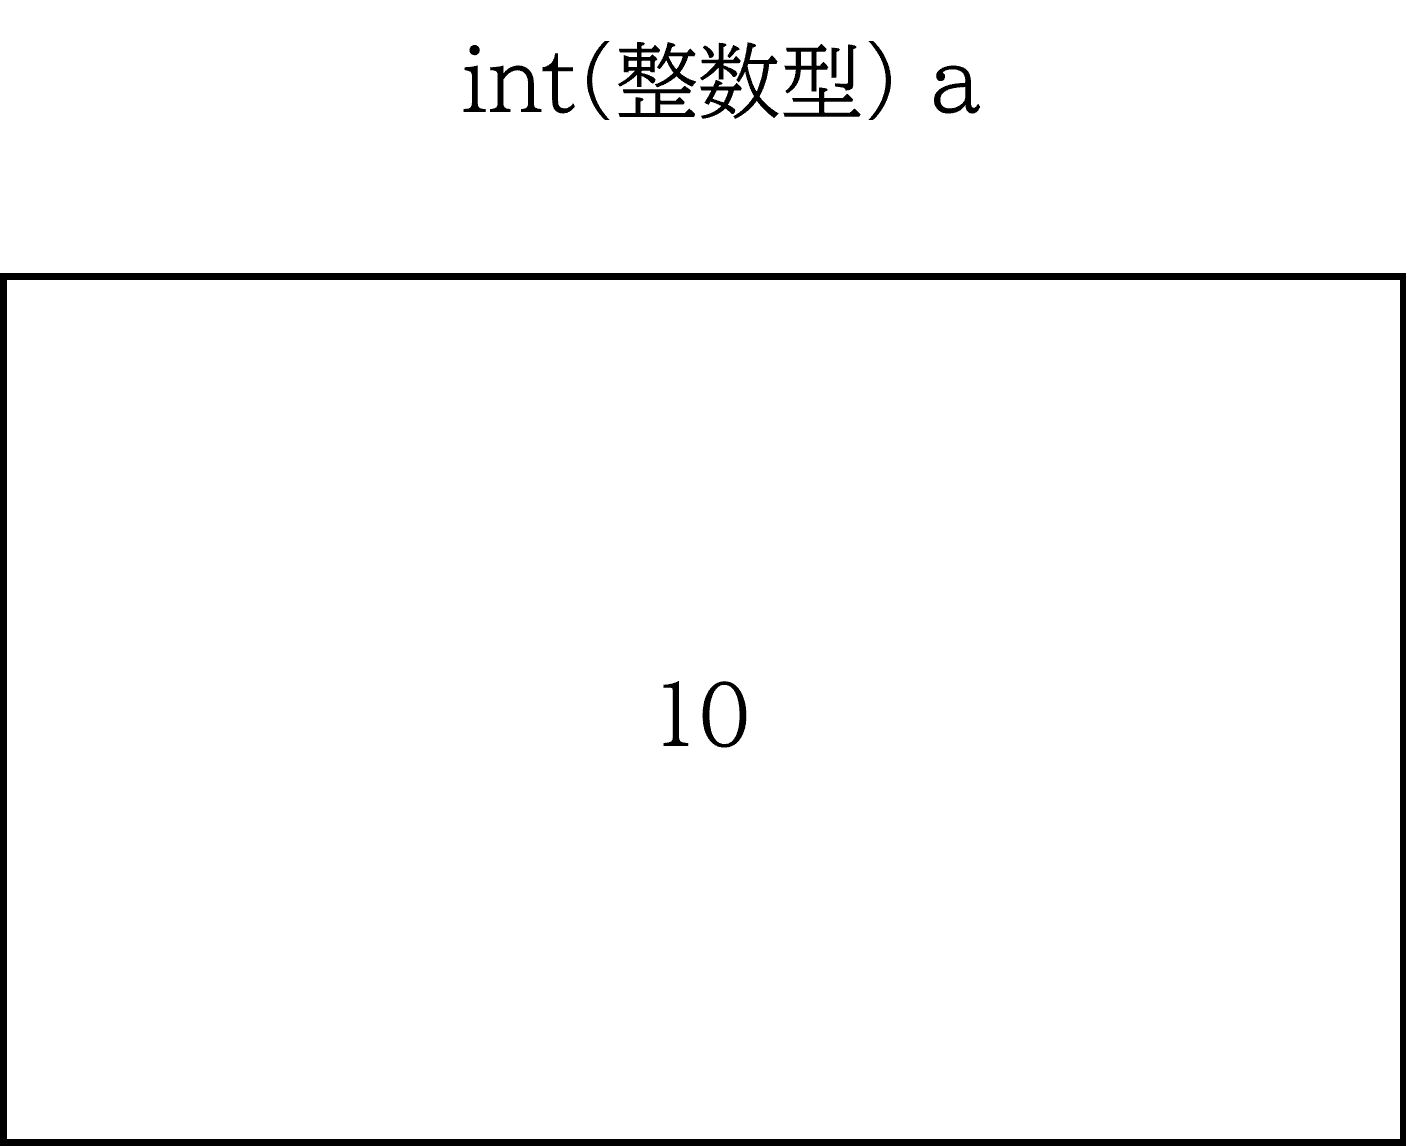
\includegraphics[width=0.6\columnwidth]{png/var.png}
                \caption{変数}
            \end{figure}
        \end{column}
        \begin{column}{0.48 \linewidth}
            \begin{figure}[b]
                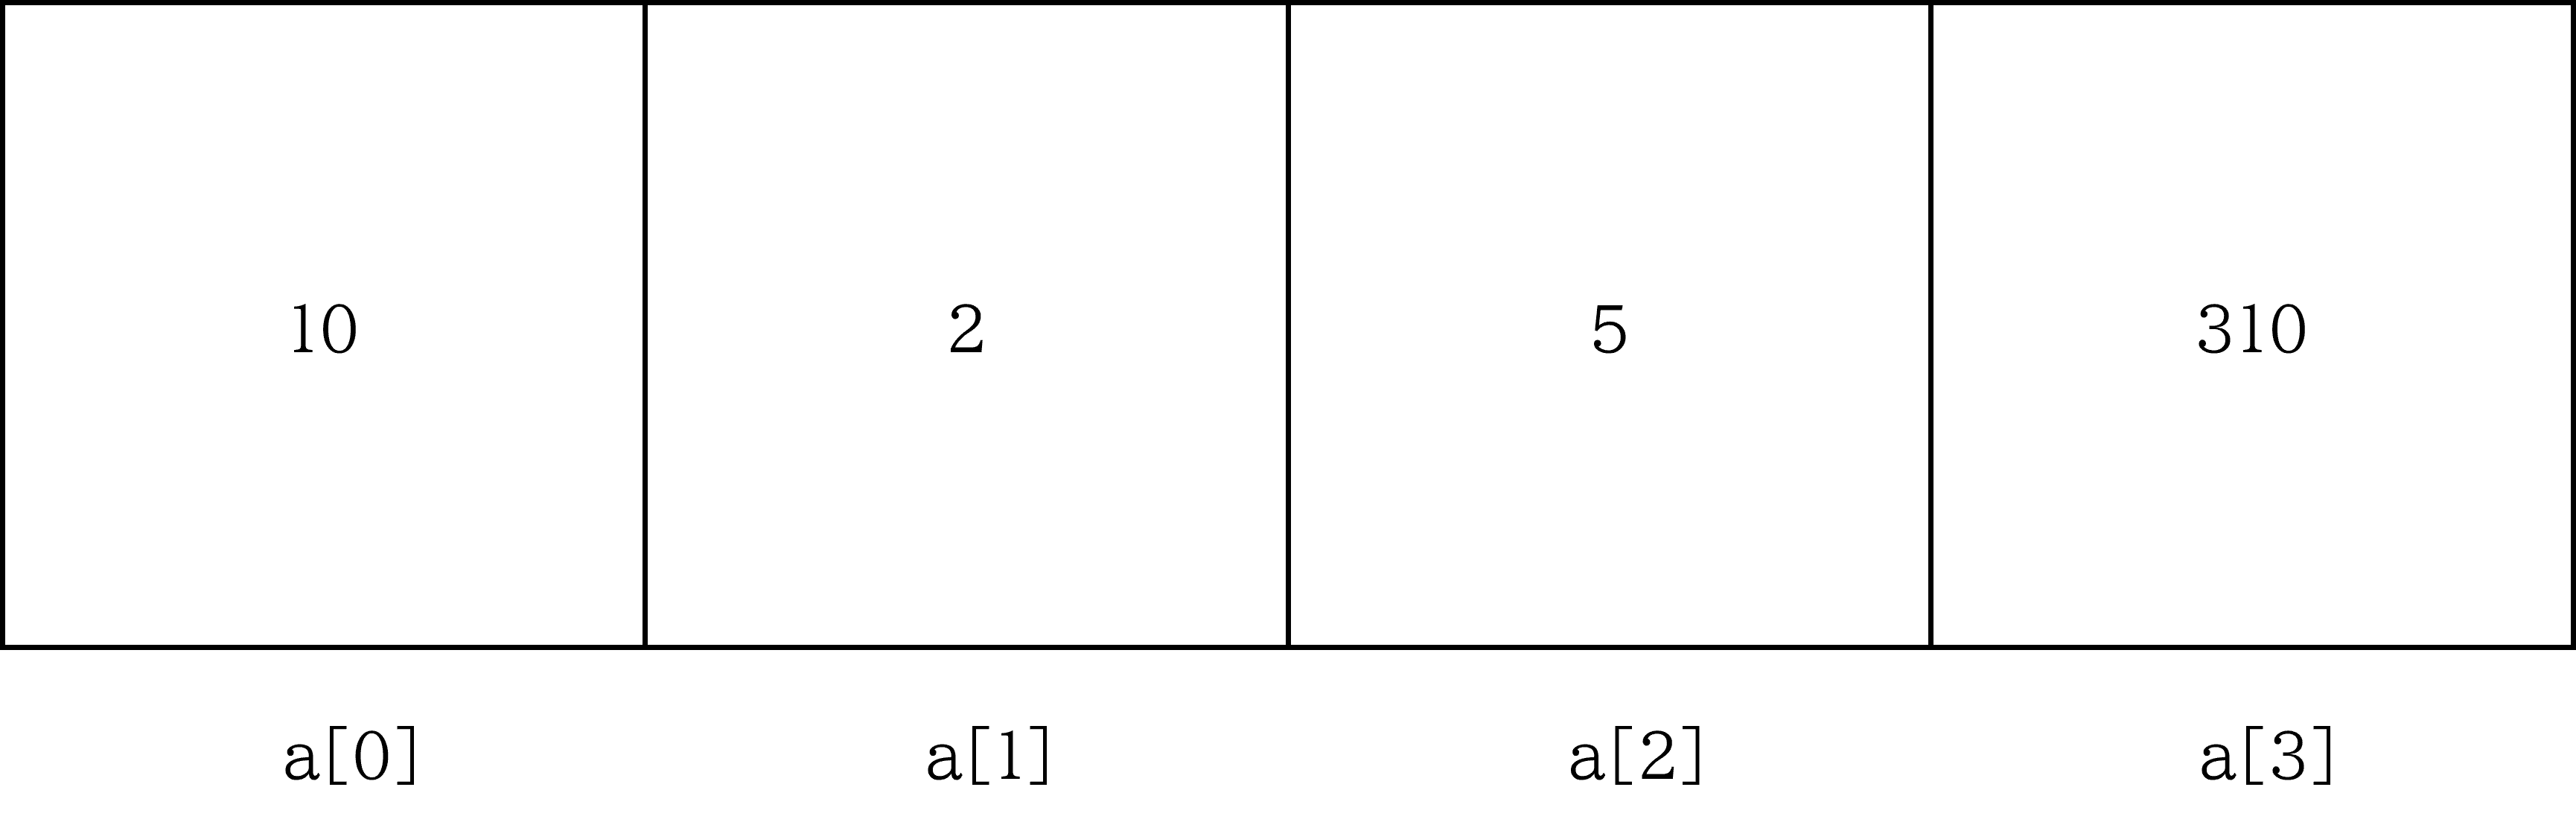
\includegraphics[width=0.6\columnwidth]{png/arr.png}
                \caption{配列}
            \end{figure}
        \end{column}
    \end{columns}
    \newpage

    変数と配列の違いは「データがメモリ上に一列に並べられているかどうかである.」\footnote{イメージとしては\ref{配列とポインタの関係性}ページのような感じ}変数の場合は,メモリ上にバラバラに存在しているが配列は一列に並んでいる.そのため,配列を用いると各データへ効率よくアクセスすることができるというメリットがある.
\end{frame}

\begin{frame}{文字列}
    文字列型「String」は変数ではあるが,char\footnote{文字型}を1次元配列化したものとして考えることができる.
    string型の変数sに"ABCD"を代入したとき,以下のように考えることができる.\footnote{実際に,s[0]とプログラム上で書くと'A'のみが返ってくる.}
    \begin{figure}[h]
        \centering
        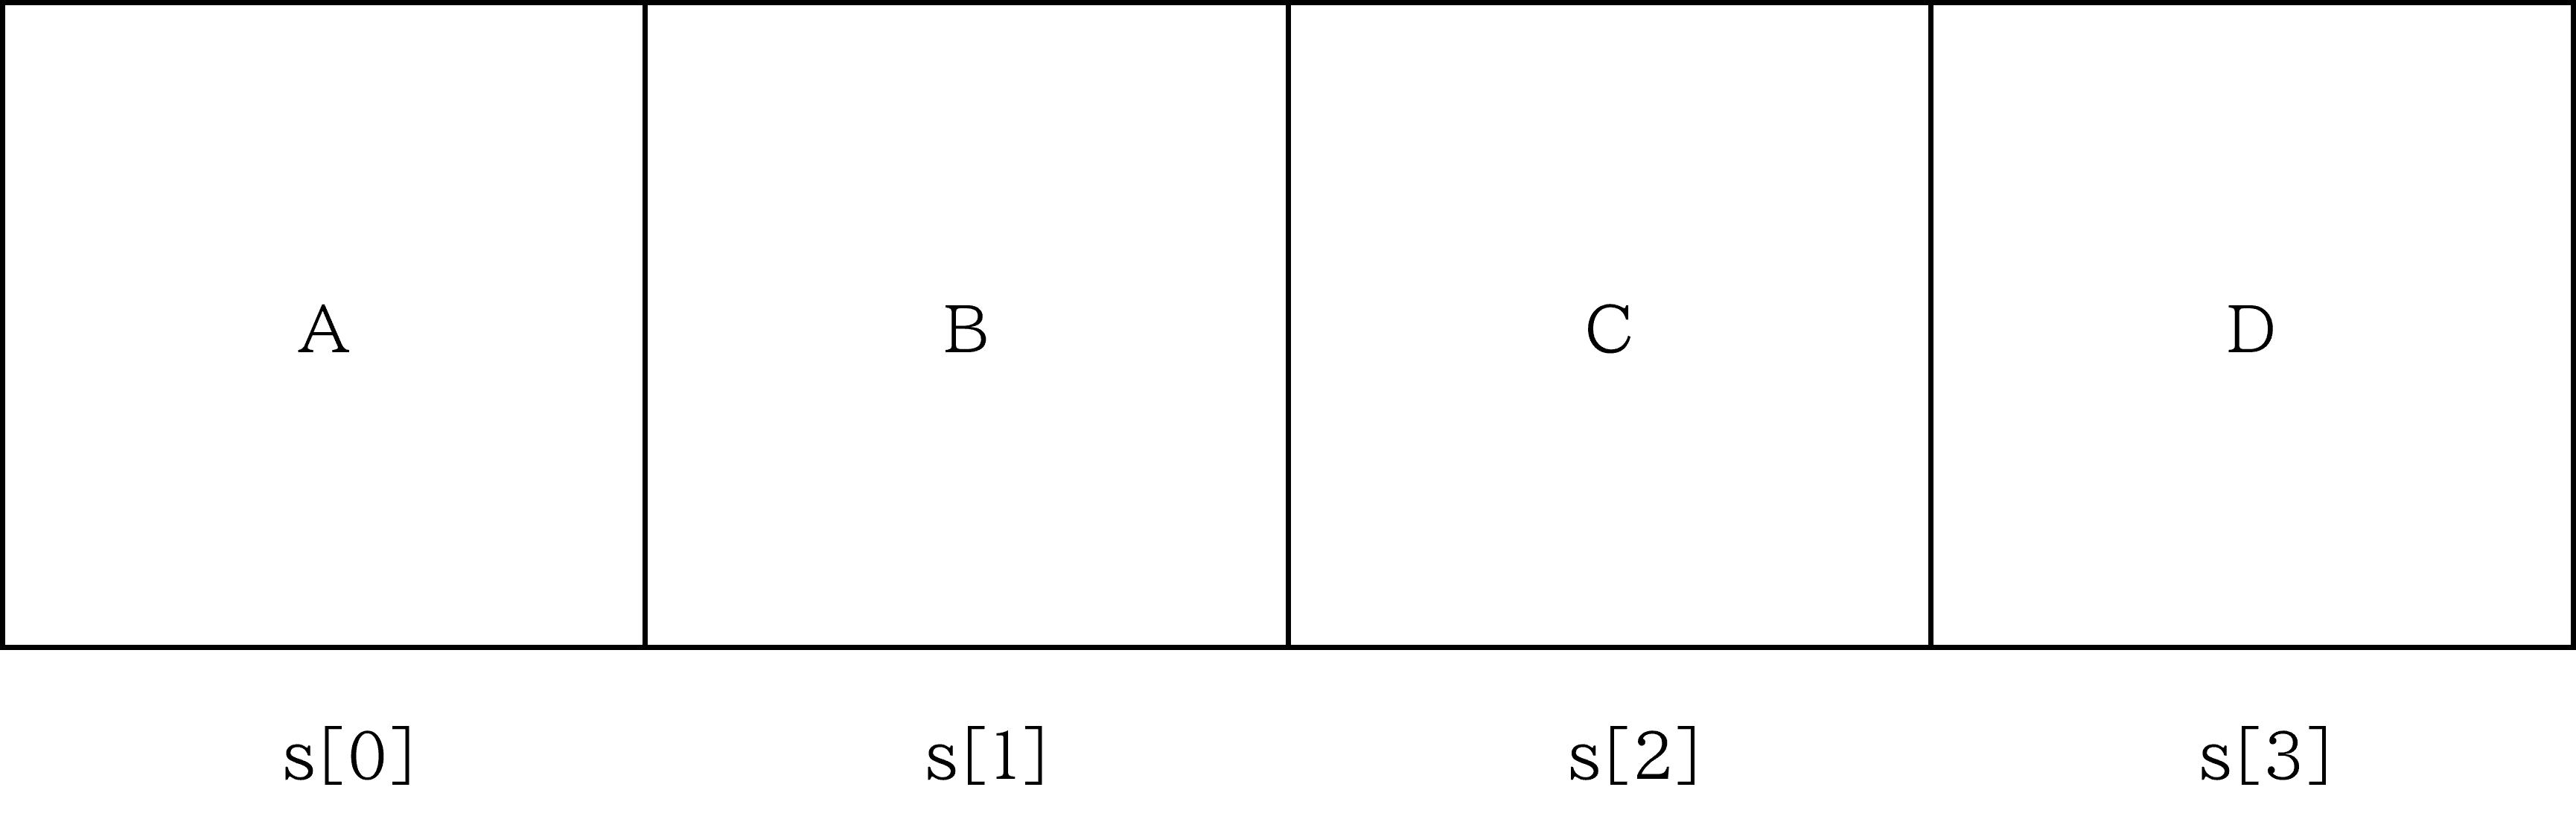
\includegraphics[width=0.4\linewidth]{png/string.png}
        \caption{char型の1次元配列}
        \label{fig:enter-label}
    \end{figure}
\end{frame}

\begin{frame}{文字列の使い方}
    文字列の使い方はC++のリファレンスを参照していただきたい.
    \url{https://cpprefjp.github.io/reference/string/basic_string.html}
    
    以下は,文字列を扱う際によく用いるものの代表例を取り上げている.
    \begin{table}[h]
        \centering
        \begin{tabular}{|l|l|}
        \hline
        名前 & 説明 \\
        \hline
        begin & 配列の要素の添え字を取得\\
        end & 最後の要素の添え字を取得\\
        \hline
        \end{tabular}
        \caption{イテレータ\footnote{ポインタと同様に扱うことができるもの.}}
        \label{tab:my_label}
    \end{table}

    \begin{table}[h]
        \centering
        \begin{tabular}{|l|l|}
        \hline
        名前 & 説明\\
        \hline
        size & 文字列の長さを取得\\
        \hline
        \end{tabular}
        \caption{領域}
        \label{tab:my_label}
    \end{table}
\end{frame}

\begin{frame}{多次元配列}
    1次元の配列だけでなく,2次元以上の配列を作成することができる.(2次元配列以上は使わなくてもプログラムを作成することは可能であるため,あまり使用しない.)
    \begin{block}{2次元配列の宣言}
        型 変数名[サイズ1][サイズ2];
        
        例として, int a[10][12];
    \end{block}
    以下は,2次元配列を視覚的に分かりやすくしたものである.
    \begin{figure}[h]
        \centering
        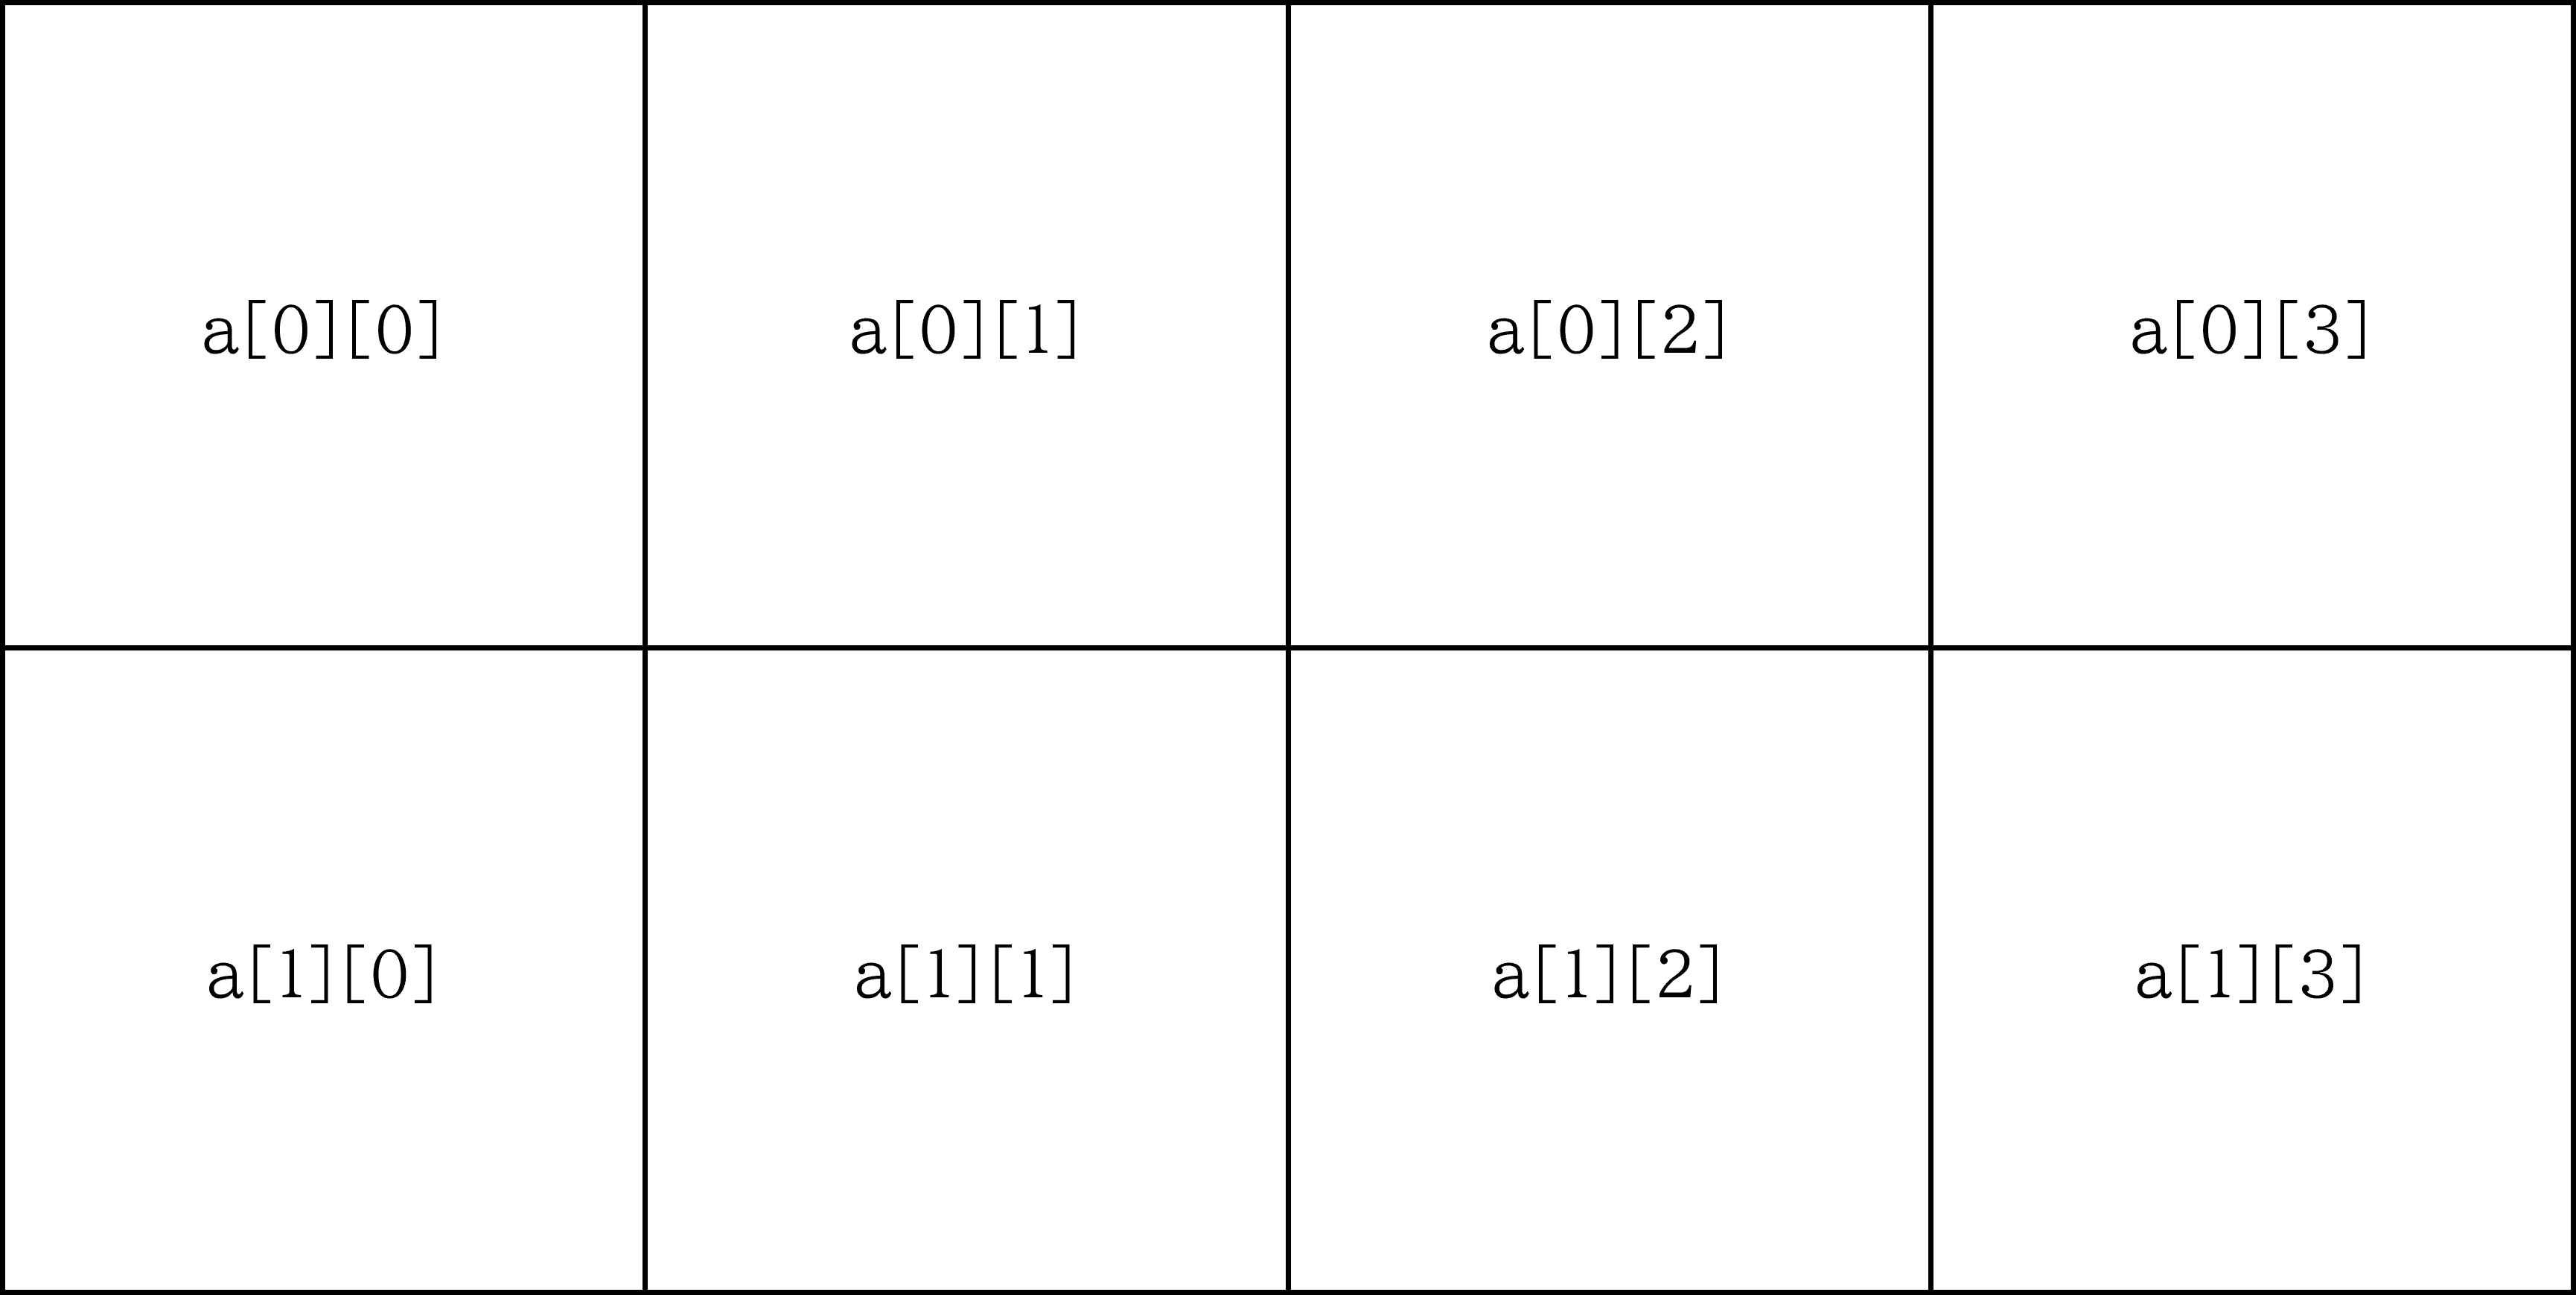
\includegraphics[width=0.4\linewidth]{png/2d_arr.png}
        \caption{2次元配列の図}
        \label{fig:enter-label}
    \end{figure}
\end{frame}

\begin{frame}{2次元配列の初期化}
    2次元配列の初期化も1次元配列と同様に初期化することができる.
    \begin{block}{2次元配列の初期化}
        型 配列名[サイズ] = \{\{値のリスト1\}, \{値のリスト2\} $\cdots$\};
        
        例として, int a[2][2] = \{\{1, 2\}, \{1, 3\}\}

    \end{block}
\end{frame}

\begin{frame}[fragile, allowframebreaks]{配列とfor文との組み合わせ}
    配列が一番有効活用できるときは,for文等の繰り返し処理を行う文法と組み合わせて使うときである.
    以下に,その例を挙げる.
    \begin{minipage}{\linewidth}
        \lstinputlisting[caption=arr\_for.cpp,label=arr]{code/arr_for.cpp}
    \end{minipage}

    \newpage

    ソースコード\ref{arr}はサイズがnの配列にn回,for文を回すことにより,配列aの全要素に値を入れることができる.これは
    \begin{enumerate}
        \item n個の変数を一度に宣言し,
        \item n個の変数にfor文を回すだけで値を代入することができる
    \end{enumerate}
    ということができ,大量のデータを扱うことができるようになるのでぜひ使えるようにしていきたい.
\end{frame}

\subsection{可変長配列}
\begin{frame}{可変長配列"vector"}
    今までの配列は最初にサイズを指定した後にサイズを変更することができなかった固定長配列というものである.しかし,プログラムの実行途中に配列の要素の増減を行いたい場合も出てくる.そのような場合に,この可変長配列「vector」を用いる.
    \begin{block}{可変長配列とは}
        プログラミングで用いられる配列変数の一種であり,配列のサイズが固定されておらず,実行途中の必要に応じて要素を追加,削除することができる配列である.
    \end{block}
    \begin{alertblock}{可変長配列を使用する際の注意点}
        可変長配列「vector」を用いる場合には,
        ヘッダーファイルにvectorを追加しなければならない.\footnote{ヘッダーファイルがbits/stdc++.hなら不要.}
    \end{alertblock}
\end{frame}

\begin{frame}{vectorの宣言}
    vectorの宣言は通常の配列とは異なるので注意する必要がある.
    \begin{block}{vectorの宣言}
    vector<型> 変数名(最初の要素数);

    例として, vector<int> a(10);
    \end{block}
\end{frame}

\begin{frame}{vectorの初期化}
    vectorの初期化は固定長配列と同様に行ってもよいが,すべての要素に同じ値を代入したい場合は本項のやり方がおすすめである.
    \begin{block}{vectorの初期化}
        vector<型> 配列名(要素数,初期値);

        例として,vector<int> a(10, 1\footnote{a[0] $\sim$ a[9]までに1が代入される.});
    \end{block}
    この方法を用いることでfor文を回すことなく配列を初期化することができる.
    
\end{frame}

\begin{frame}{vectorの使い方}
    vectorの使い方についてはC++のリファレンスを参照していただきたい.
    \url{https://cpprefjp.github.io/reference/vector/vector.html}
    
    以下は,vectorを扱う際によく用いるものの代表例を挙げている.
    \begin{table}[h]
        \centering
        \begin{tabular}{|l|l|}
            \hline
            名前 & 説明\\
            \hline
            push\_back & 末尾へ要素を追加\\
            pop\_back & 末尾から要素を削除\\
            insert & 要素の挿入\\
            \hline
        \end{tabular}
        \caption{コンテナの変更}
        \label{tab:my_label}
    \end{table}
\end{frame}

\section{ポインタ}
\begin{frame}[fragile]{ポインタの使用例}
    ここでは,ポインタの簡単な使い方について以下のソースコードを記述する.
    \lstinputlisting[label=point.cpp]{code/point.cpp}
\end{frame}

\begin{frame}[allowframebreaks]{ポインタとは}
    \begin{alertblock}{}
        ポインタは難しい分野のため,徐々に理解していけばそれで充分である.
    \end{alertblock}
    \begin{block}{ポインタとは}
        ポインタとは,変数等がメモリのどの場所に保存されているかを指し示す仕組みである.つまり,データ本体ではなく,それがある場所のことである.
    \end{block}
    \begin{block}{ポインタの宣言}
        型 *変数名;

        例として, int *p;
    \end{block}
    \begin{block}{ポインタ演算子}
        ポインタを用いる際にはポインタ演算子というものを用いる.
        ここでは, pをポインタ変数として扱う.
        \begin{table}[h]
            \centering
            \begin{tabular}{|l|l|}
                \hline
                演算子(変数そのもの) & 説明\\
                \hline
                p & アドレス自体を意味\\
                *p & アドレスが指し示す値\\
                \&q (qはただの変数) & qが保存されているアドレスを指し示す\\
                \hline
            \end{tabular}
            \caption{ポインタ演算子}
            \label{tab:my_label}
        \end{table}
    \end{block}

    \begin{figure}[h]
        \centering
        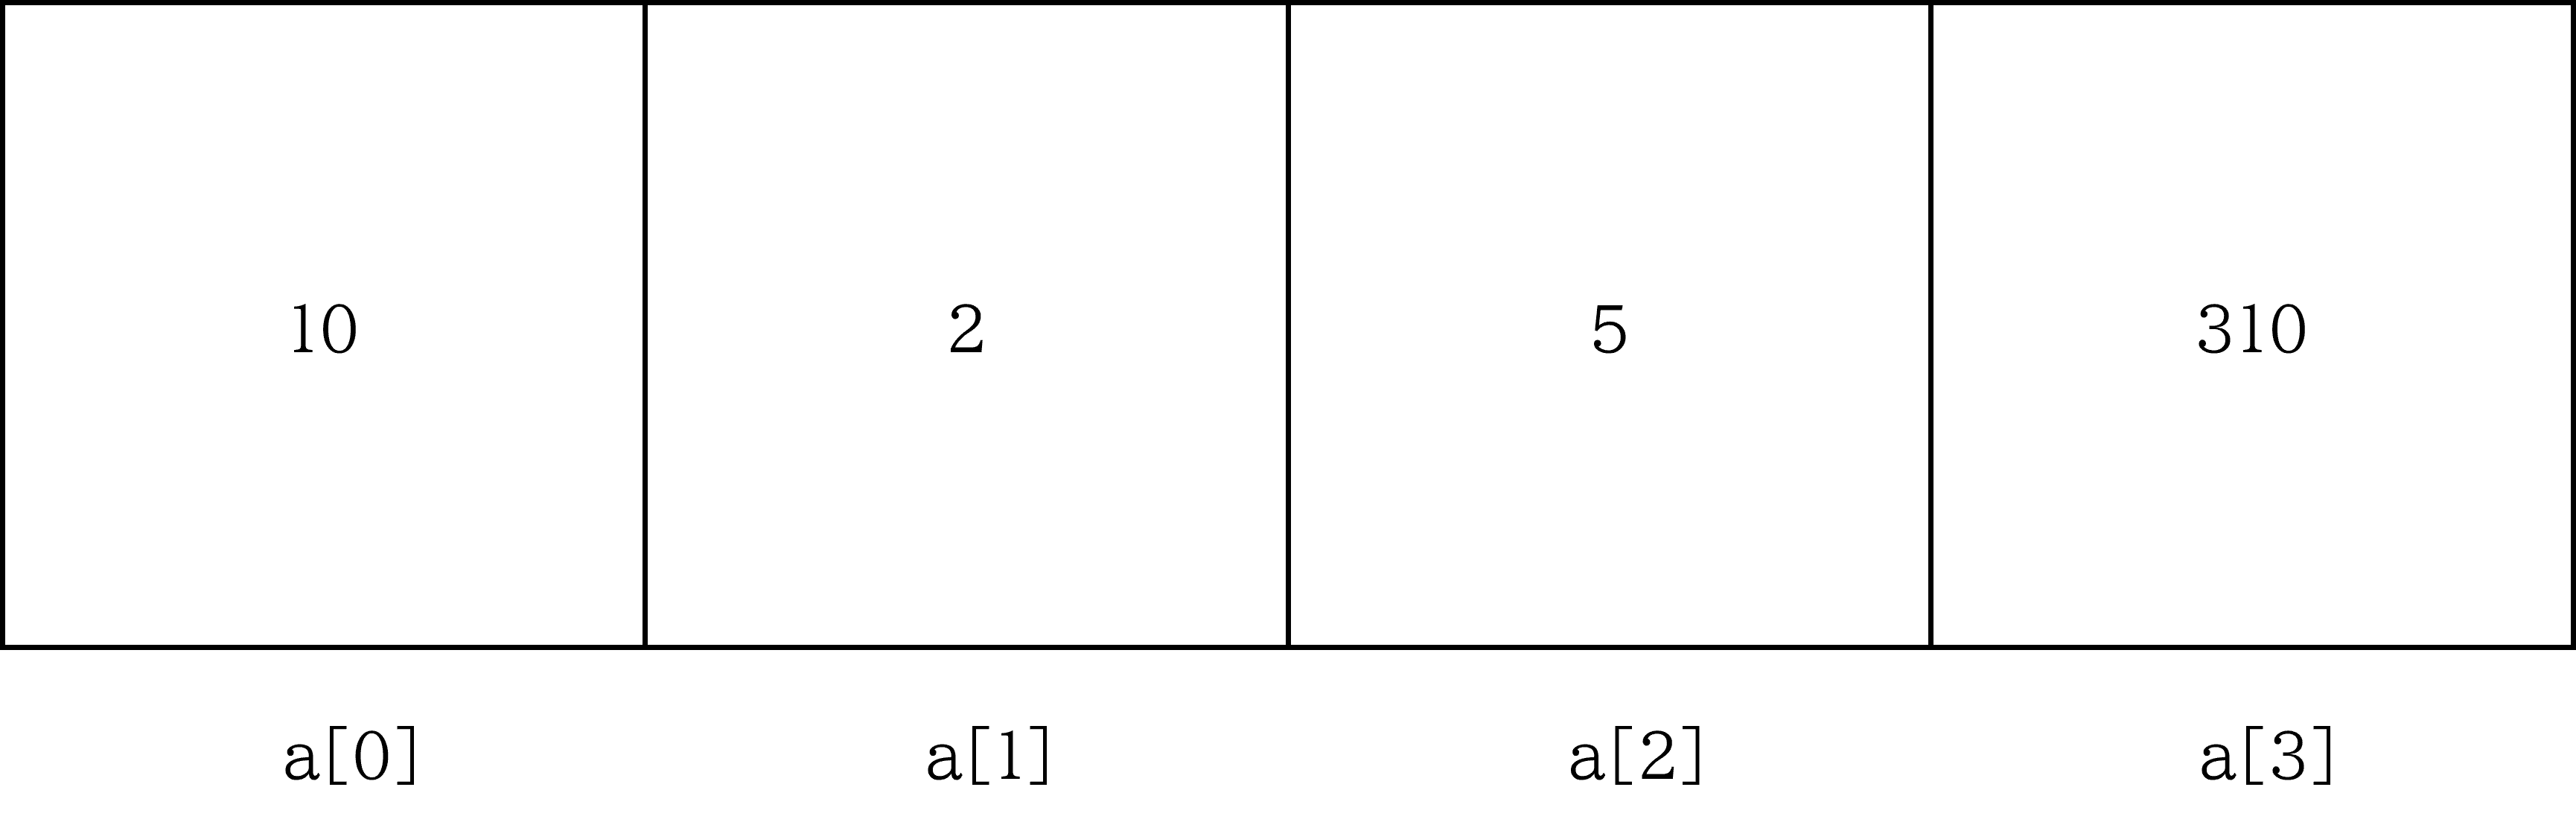
\includegraphics[width=0.4\linewidth]{png/arr.png}
        \caption{配列とポインタの関係性}
        \label{fig:enter-label}
    \end{figure}
\end{frame}

\begin{frame}{ポインタの演算制限について}
    \begin{block}{ポインタの演算制限}
        ポインタでは整数の加算と減算以外は実行することができない.即ち,ポインタ変数に適用できる演算は以下の6つのみである.

        \centering
            *, \&, +, ++, -, --
    \end{block}
    \begin{alertblock}{ポインタ変数でのインクリメント,デクリメント}
        ポインタ変数で*p++としたとき,ポインタが指している値ではなく,ポインタ自体をインクリメントしている.ポインタが指している値をインクリメントしたい場合は,(*p)++とするのが正解である.

    \end{alertblock}
\end{frame}

\subsection{配列とポインタ}
\begin{frame}[fragile, allowframebreaks]{配列とポインタの関係性} \label{配列とポインタの関係性}
ポインタと配列はとても密接に関わりあっている.
\begin{block}{配列とポインタの関係}
    添え字をつけずに配列名の場合は,配列の先頭を指すポインタとなってしまう.そのため,変数として配列を扱いたい場合は添え字を忘れてはいけない.
\end{block}
    \begin{minipage}{\linewidth}
        \lstinputlisting[caption=p.cpp]{code/p.cpp}
    \end{minipage}

\newpage

    \begin{figure}[h]
        \centering
        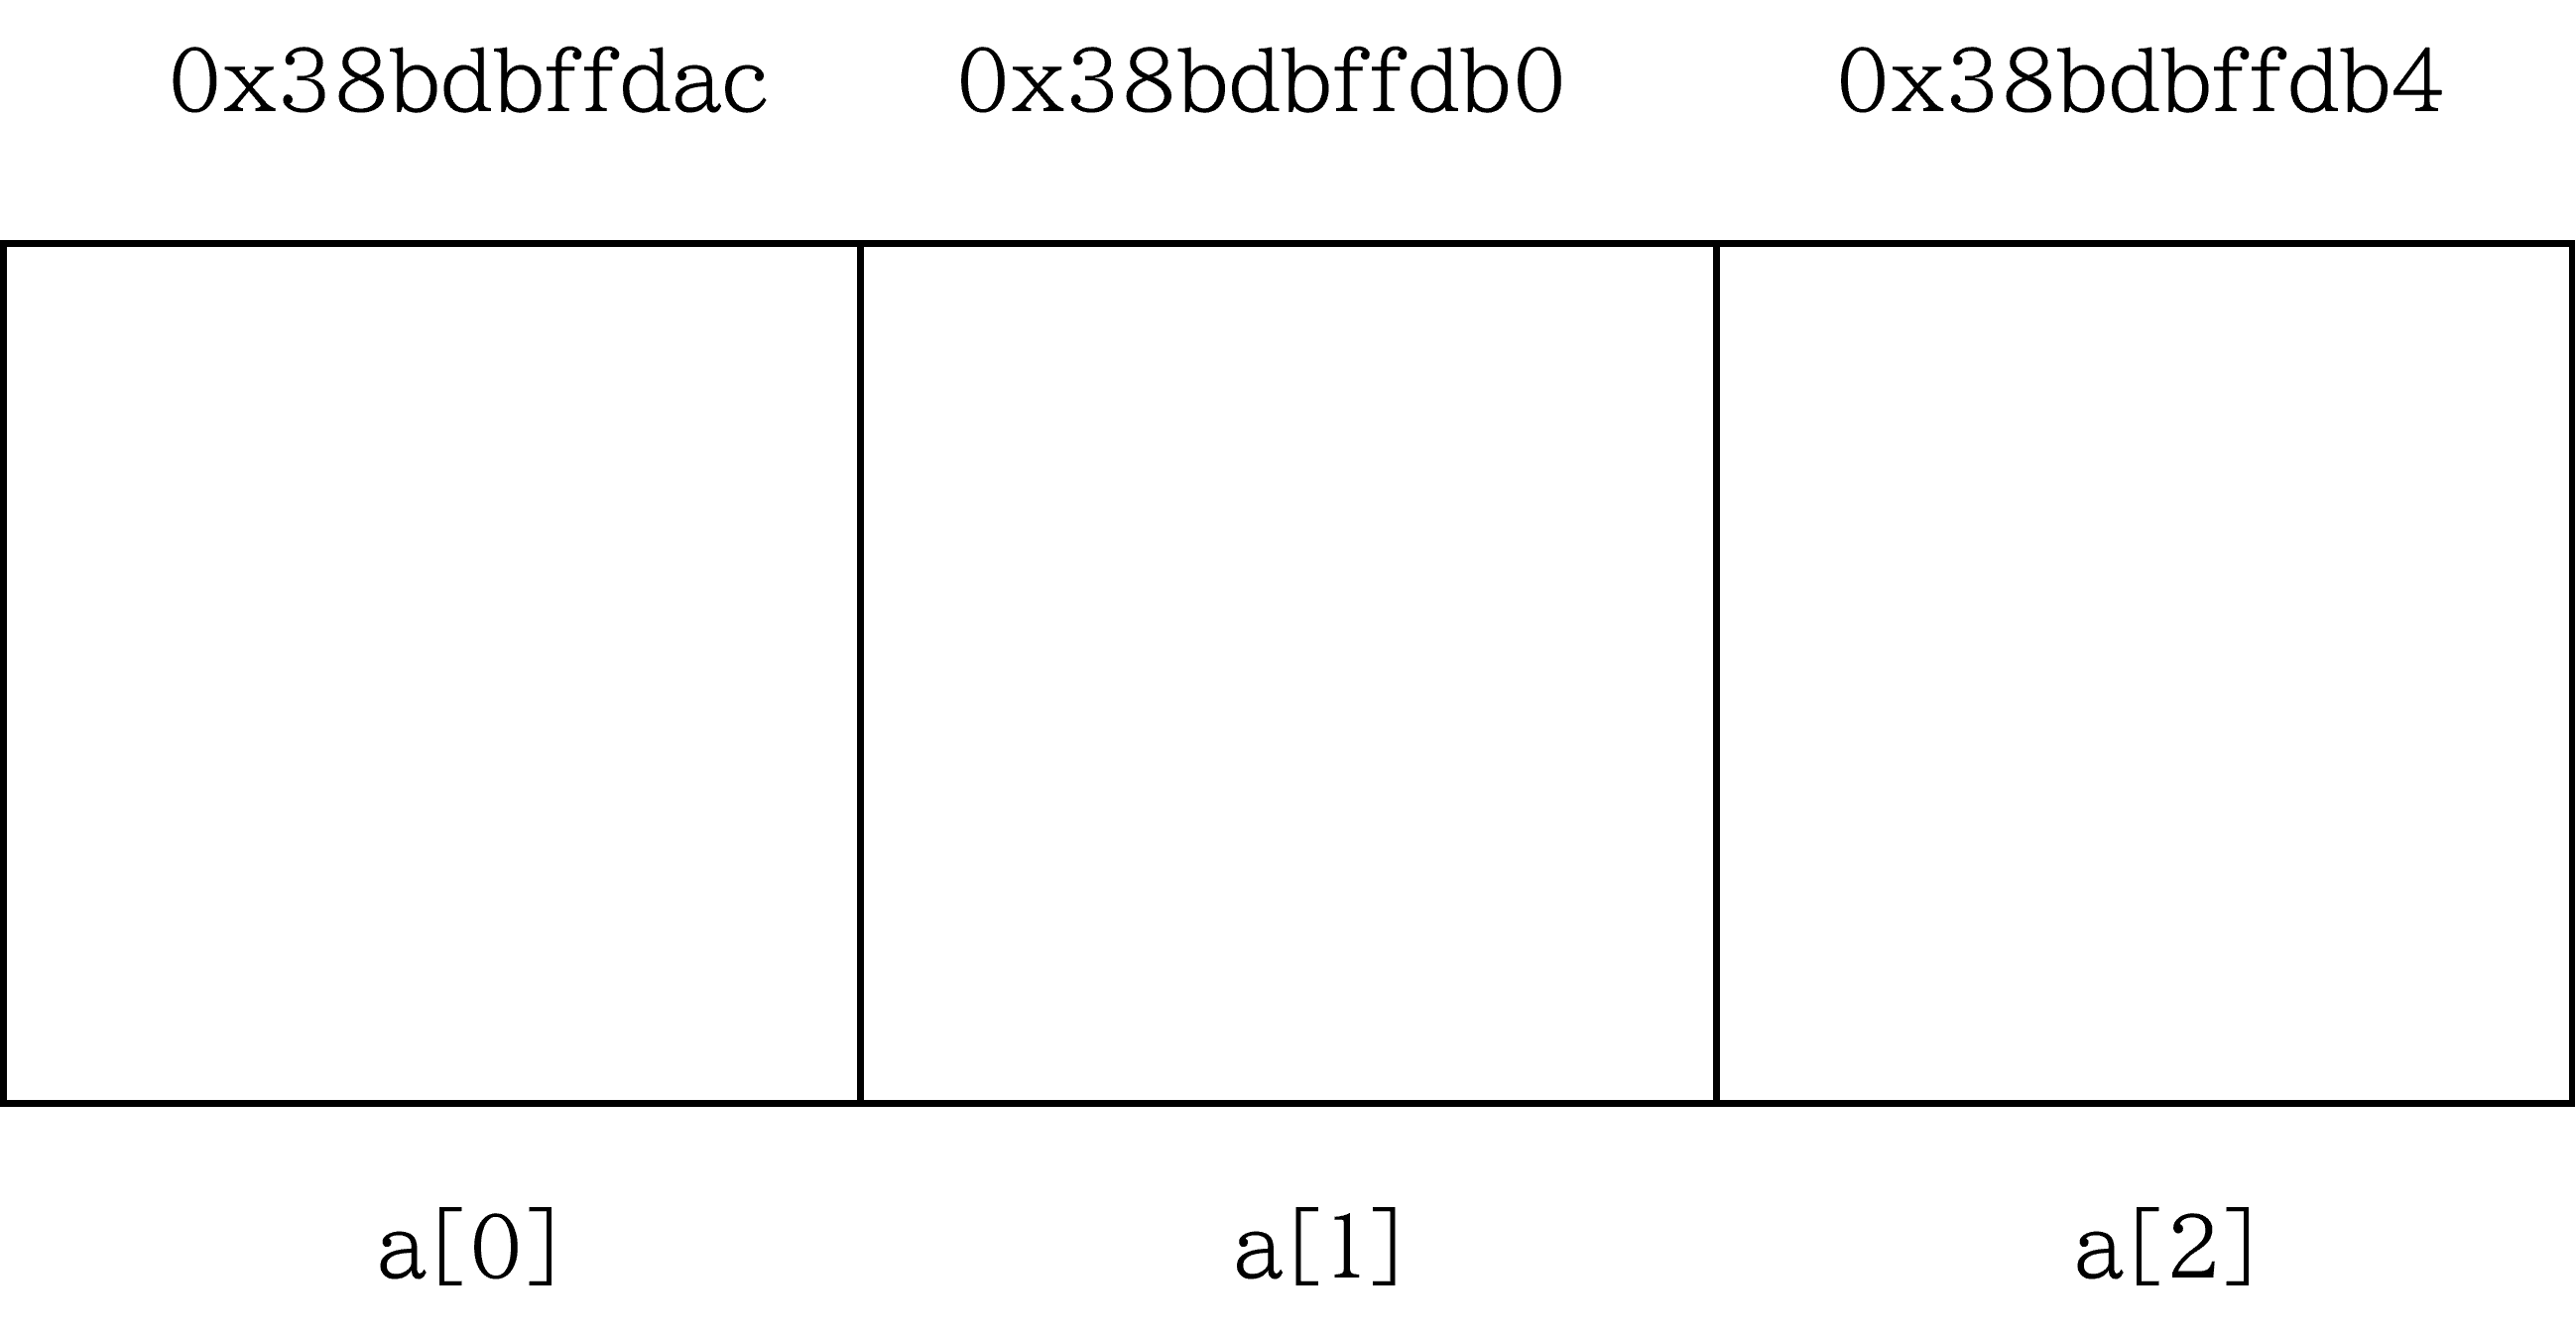
\includegraphics[width=0.5\linewidth]{png/arr_p.png}
        \caption{配列とポインタの関係性}
        \label{fig:enter-label}
    \end{figure}
\end{frame}

\begin{frame}[fragile]{多重間接参照}
    \begin{block}{多重間接参照とは}
        ポインタを使い別のポインタを指すことができる.その場合,最初のポインタは2番目のポインタのアドレスを持ち,2番目のポインタは変数を指す.しかし,多重間接参照は連鎖をたどるのが面倒なため極力使用は避けたい.
    \end{block}

    \begin{figure}[h]
        \centering
        
\includegraphics[width=0.5\linewidth]{png/multi.png}
        \caption{多重間接参照の図}
        \label{fig:enter-label}
    \end{figure}
\end{frame}

\section{関数}
\begin{frame}{関数とは}
    \begin{block}{関数とは}
         ある処理をまとめて名前を付けたものを関数と呼ぶ.
    \end{block}
    \begin{block}{関数を使うメリット}
        関数を使うことによってコードの重複を減らせることができることが理由である.
    \end{block}
\end{frame}

\begin{frame}[fragile]{main関数}\label{main}
    \lstinputlisting[caption=main関数]{code/main.txt}
    main関数とは各ソースコードに存在する特別な関数である.
    この関数はプログラム実行時にシステムから呼び出される.また,return 0;に到達するとその時点でプログラムを終了する.
\end{frame}
\begin{frame}{関数について}
    関数は以下の二つに分けることができる.
    \begin{enumerate}
        \item ユーザー定義型関数
        \item 標準関数
    \end{enumerate}
    \begin{block}{ユーザー定義型関数}
        この関数は,プログラマーがそのコードの中で作成し,実行する関数である.必要になったタイミングで関数を作って使うことができる.
    \end{block}
    \begin{block}{標準関数}
       この関数は,ヘッダーファイル等に最初から入っている関数である.そのため,プログラマーが実際に作成することなく使えることができる.ただし,ヘッダーファイルを読み込んでいない場合エラーが発生するので注意すること. 
    \end{block}
    ユーザー定義型関数を作成する際には基本的には以下の二つが必要となる.
    \begin{enumerate}
        \item 関数プロトタイプ\footnote{関数定義がmain関数前であれば必要はない}
        \item 関数定義
    \end{enumerate}
\end{frame}

\begin{frame}[fragile]{関数の使用例}
    ここでは,関数を用いた際の全体の流れとして以下のコードを記述する.
    \begin{minipage}{\linewidth}
        \lstinputlisting[caption=func.cpp, label=関数使用例]{code/func.cpp}
    \end{minipage}
    次項から,詳しい解説を行っていく.
\end{frame}

\subsection{関数プロトタイプ}
\begin{frame}{関数プロトタイプ宣言について}
    \begin{block}{関数プロトタイプ宣言とは}
        関数定義がmain関数の後の場合,ファイルをコンパイルする際にコンパイラに対して関数の情報を渡さないまま関数を呼び出してしまう.そのため関数を呼び出した際にその呼び出し方に誤りがないか確認するための宣言である.

        (関数定義がmain関数前に行っておけば,プロトタイプ宣言は必要ない.)
    \end{block}
    プロトタイプ宣言には以下の3つの役割を果たしている.
    \begin{enumerate}
        \item 関数の戻り値の型をコンパイルに伝えること
        \item 関数を呼び出すために使用した引数の型と仮引数の宣言時の型との間で不正確な型変換が行われたとき,コンパイラが検出して報告できるようにしている.
        \item 関数に渡した引数の数が関数の仮引数の数と一致しない場合にも報告できるようにしている.
    \end{enumerate}
\end{frame}

\begin{frame}[fragile]{関数プロトタイプの宣言}
    \begin{block}{}
        返り値の型 関数名 (仮引数リスト);        
    \end{block}
    
    関数のプロトタイプ宣言の一般形は上に書いてある書き方である.
    
    また,引数は可変個にすることができるが使用することはない為,宣言の方法だけ触れておく.
    \begin{block}{}
        int func (int i, ...);
    \end{block}
\end{frame}

\subsection{関数定義}
\begin{frame}[fragile]{関数定義}
\lstinputlisting[caption={関数定義}]{code/func.txt}
関数定義には以下の要素が必要である.
\begin{enumerate}
    \item 戻り値の型
    \item 関数名
    \item 引数リスト
    \item 実際に行う処理
    \item 戻り値
\end{enumerate}
次項から各項目について解説していく.
\end{frame}

\begin{frame}{戻り値の型}
    \begin{block}{戻り値の型}
        戻り値の型は,関数が値を返す\footnote{戻り値については後で詳しく解説する.}際のデータ型のことである.
    \end{block}
    \begin{exampleblock}{再掲}
        \begin{table}[]
            \centering
            \begin{tabular}{|l|l|l|}
                \hline
                型       & キーワード  & サイズ\\
                \hline
                文字データ & char  & 1バイト\\
                符号付き整数 & int  & 2バイト\\
                浮動小数点 & float & 4バイト\\
                倍精度浮動小数点 & double & 8バイト\\
                値なし & void & \\
                \hline
            \end{tabular}
            \caption{基本のデータ型}
            \label{tab:my_label}
        \end{table}        
    \end{exampleblock}
\end{frame}

\begin{frame}[fragile]{引数リスト}
    \begin{block}{引数とは}
        関数を呼び出した際に関数に対して渡す値.引数の宣言は通常の変数と同様に行う.
    \end{block}
    \lstinputlisting[caption=引数の例,label=引数]{code/arg.txt}
    ソースコード\ref{引数}では,1行目の()で引数を宣言している.関数を呼び出して使用する際は必ず関数名の後ろに渡したい値を記述しなければならないので注意すること.
\end{frame}

\begin{frame}[fragile]{戻り値}
\begin{block}{戻り値とは}
    関数が処理を終えた後に返す.
    関数の最後にあるreturn 戻り値で値を返すことができる.
\end{block}
    \lstinputlisting[caption=戻り値の例, label=戻り値]{code/rv.txt}
    ソースコード\ref{戻り値}では,関数の中にreturn a;と書いているため,この関数が呼び出されたときにaが返り値として返る.
\end{frame}

\subsection{引数の値渡しと参照渡し}
\begin{frame}[fragile]{値渡しと参照渡し}
    関数に引数を渡す場合,以下の2つの方法がある.
    \begin{enumerate}
        \item 値渡し
        \item 参照渡し
    \end{enumerate}
    1つ目の値渡しとは,引数に値がコピーされる.なので,呼び出し元の値は影響を受けない.2つ目の参照渡しでは,アドレスが引数にコピーされる.そのため,呼び出された関数で値を変更すると呼び出し元の値も変更される.
    \lstinputlisting[caption=参照渡しの例, label=参照渡し]{code/pass.txt}
    ソースコード\ref{参照渡し}では,関数に2つの変数のポインタを渡しているので引数が指す実際の値が入れ替わる.
\end{frame}
\section{再帰}
\begin{frame}[fragile]{再帰の使用例}
ここでは,再帰の全体像を確認するために以下のコードを記述しておく.
    \begin{minipage}{\linewidth}
        \lstinputlisting[caption=reur.cpp]{code/reur.cpp}
    \end{minipage}
\end{frame}
\begin{frame}[fragile]{再帰とは}
    \begin{alertblock}{}
        再帰関数は非常に難しい分野のため,無理に理解しようとする必要はない.
    \end{alertblock}
    \begin{block}{再帰とは}
        関数の中で自分自身(その関数自身)を呼び出すことを再帰と呼ぶ.
    \end{block}
    \lstinputlisting[caption=再帰の一般形の一つ, label=再帰の一般形]{code/reur.txt}
    \begin{alertblock}{}
        再帰には様々な書き方であるため,ソースコード\ref{再帰の一般形}のような書き方をしなくても良い.
    \end{alertblock}
\end{frame}

\section{構造体}

\begin{frame}[fragile]{構造体の使用例}
 以下のコードでは構造体の例である.   
    \begin{minipage}{\linewidth}
        \lstinputlisting[caption=str.cpp]{code/str.cpp}
    \end{minipage}
\end{frame}

\begin{frame}[fragile, allowframebreaks]{構造体の基礎}
    \begin{block}{構造体とは}
        構造体とは,メンバと呼ばれる互いに関連のある2つ以上の変数で構成される複合データ型である.配列は全て同じデータ型であるが,メンバはそれぞれ異なる型を持つことができる.
    \end{block}
    \lstinputlisting[caption = 構造体の定義]{code/str.txt}
    \begin{block}{構造体の変数の宣言}
        struct タグ名 変数リスト;
    \end{block}

    \newpage

    構造体型をを定義したら,後はその型の変数をいくつでも生成することができる.
    \begin{block}{構造体を用いる手順}
        構造体を用いる際の手順は以下のとおりである.
        \begin{enumerate}
            \item どんなデータを扱うのか考える.
            \item 変数として実態を作る.
            \item 実際に数値や文字を格納
        \end{enumerate}
    \end{block}    
    \begin{block}{構造体のアクセス方法}
        構造体のメンバにアクセスするためには,以下の形式で書かなければならない.

        変数名.メンバ名
    \end{block}
    \begin{exampleblock}{構造体を用いるメリット}
        構造体を用いることでプログラムを綺麗に分かりやすく記述することができる.
    \end{exampleblock}

    \newpage

    \begin{figure}[h]
        \centering
        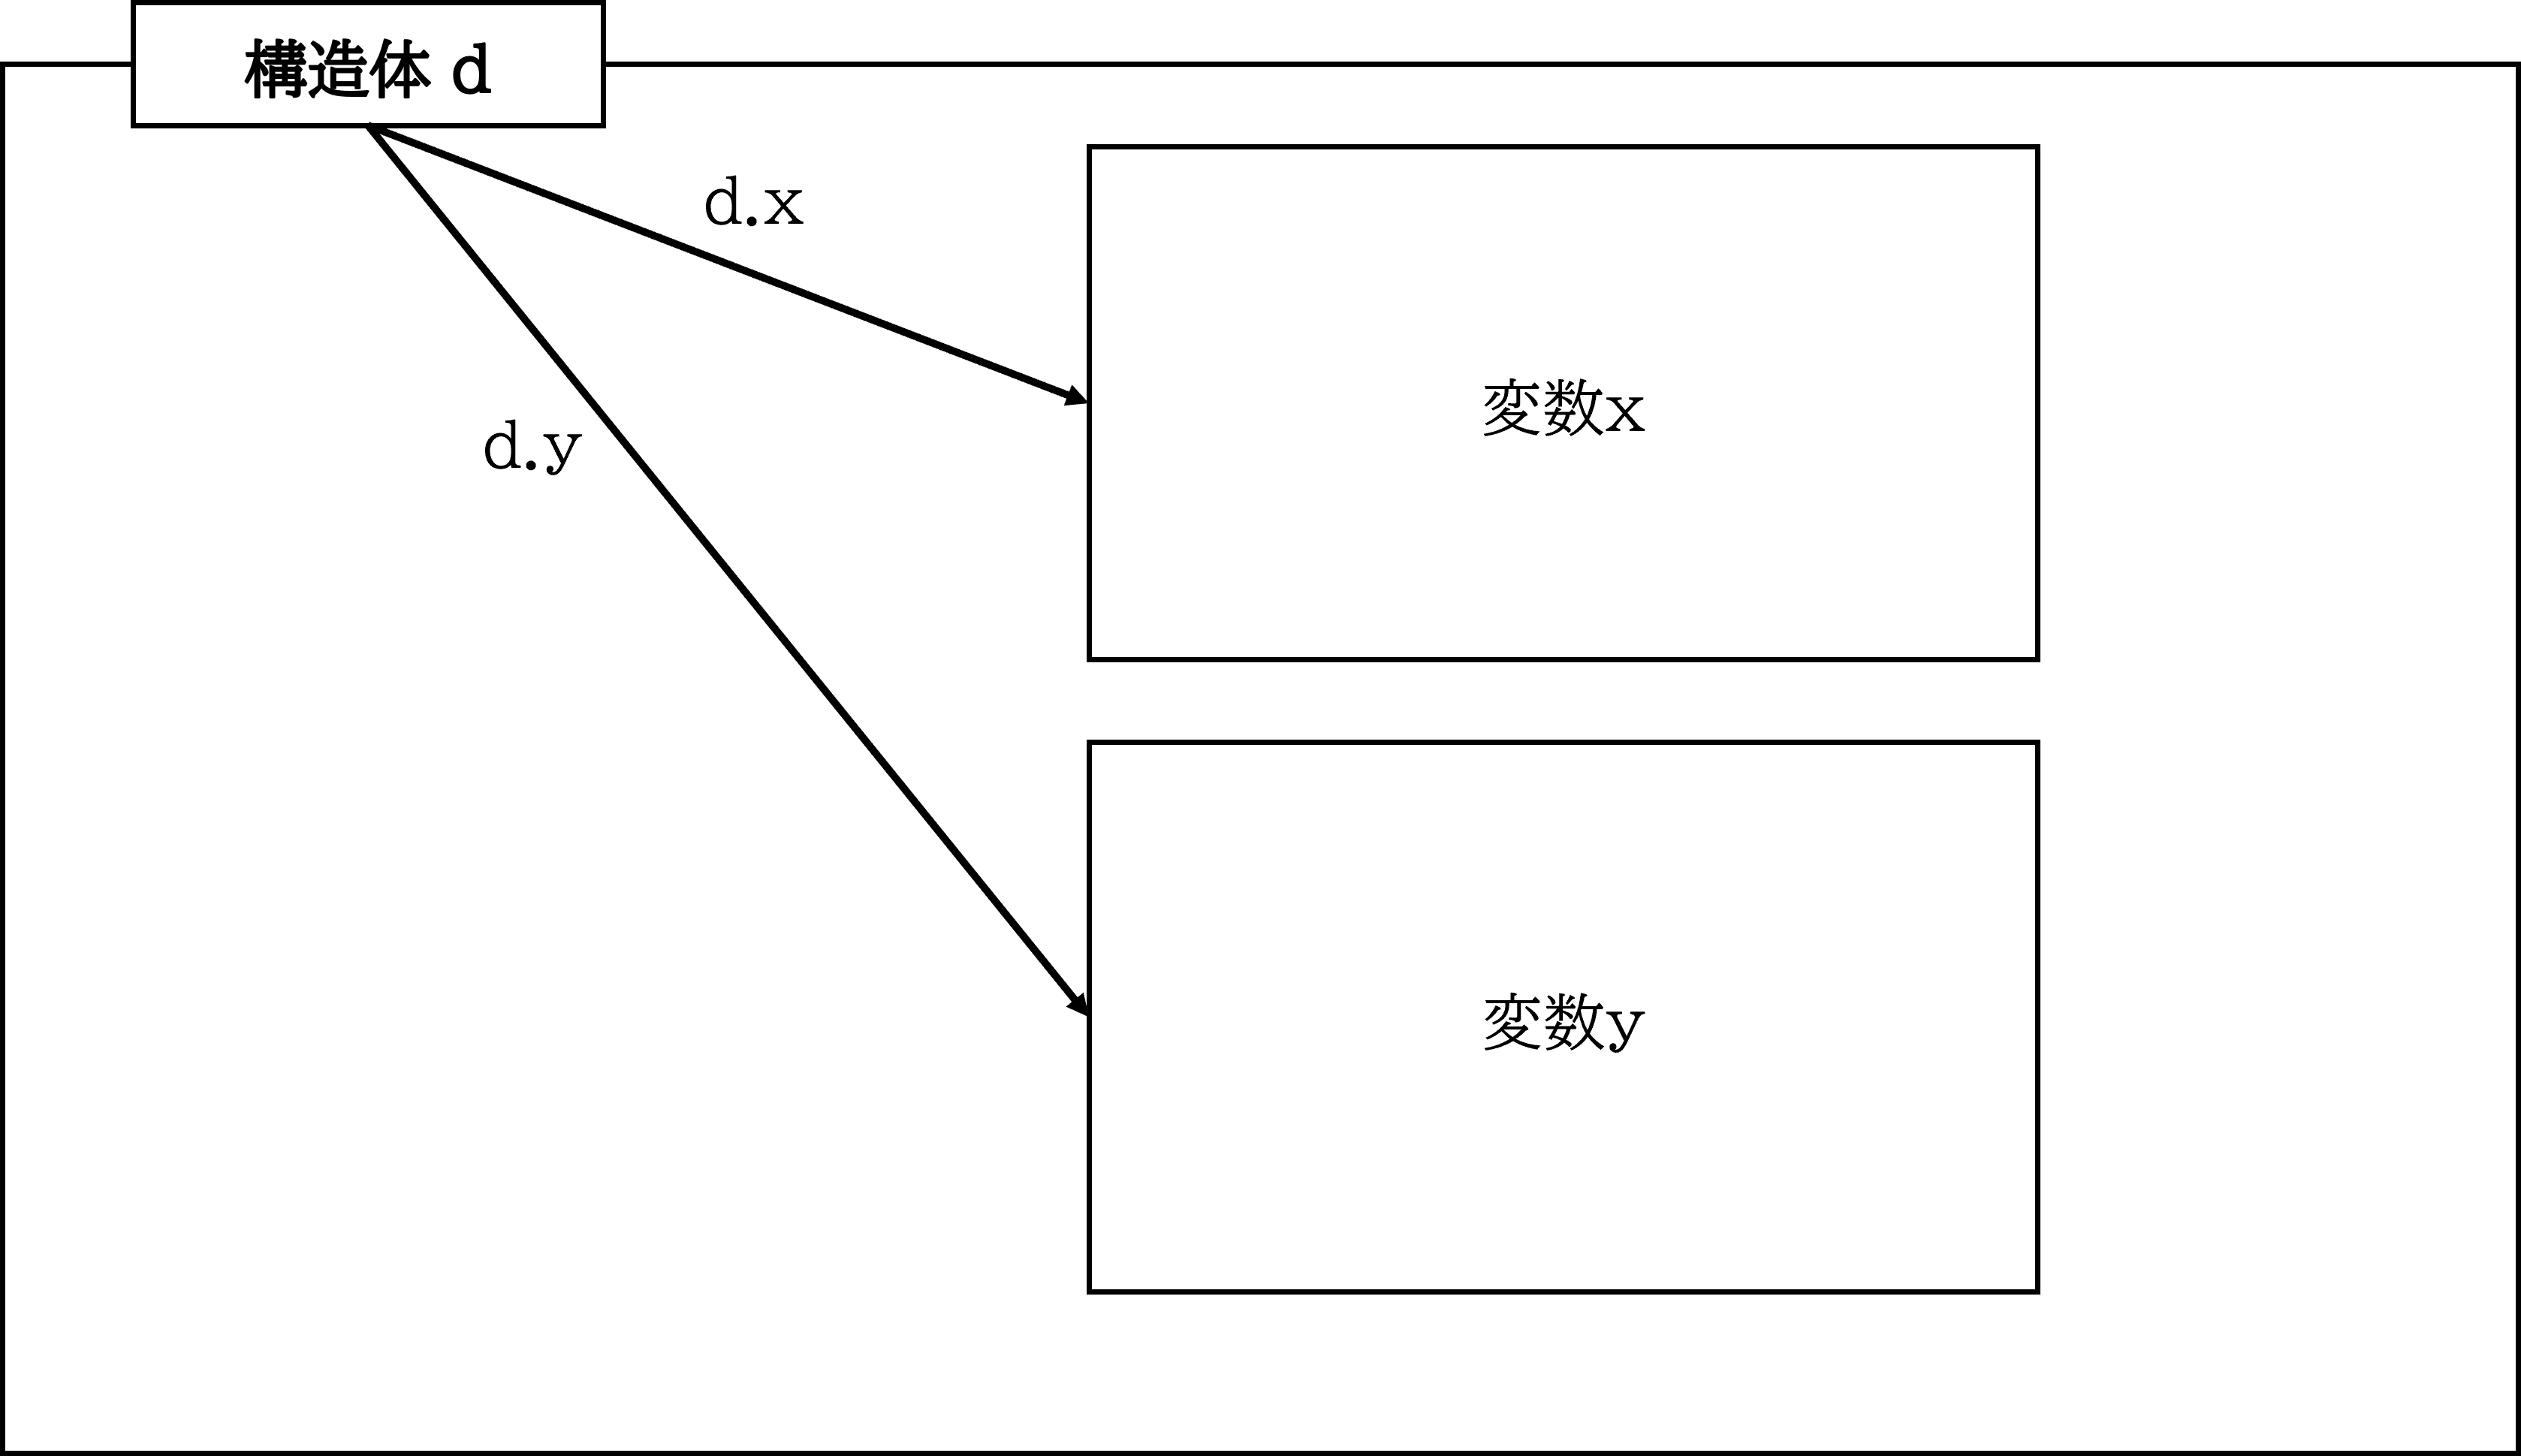
\includegraphics[width=0.5\linewidth]{png/str.png}
        \caption{構造体とメンバ変数の関係}
        \label{fig:enter-label}
    \end{figure}
\end{frame}

\begin{frame}[fragile, allowframebreaks]{構造体へのポインタ}

    \lstinputlisting[caption=str\_p.cpp]{code/str_p.cpp}

    \newpage

    \begin{block}{ポインタを介したメンバ変数へのアクセス}
    ポインタ変数 -> メンバ変数;

    上記に書いた方法をアロー演算子と呼ぶ.
\end{block}
アロー演算子を用いることでポインタを用いたプログラムを書く際,とても読みやすくなるため積極的に使用していきたい.

\lstinputlisting[caption=アロー演算子, label=アロー演算子]{code/arrow.txt}

ソースコード\ref{アロー演算子}の二つは同じ意味である.
\end{frame}

\section{参考文献}
\begin{frame}{参考文献}
    \begin{thebibliography} {99}
    \bibitem{独習}ハーバード・シルト,独習C++ 第4版 (2016)
    \bibitem{KUTPG}"KUT-PG 高知工科大学 プログラミング集団 Wiki*"
    \url{https://wikiwiki.jp/kut-pg/}
    
    (アクセス日: 2024-4-16)
    \end{thebibliography}
\end{frame}
\end{document}